\chapter{Sistema de reconocimiento de porterías}\label{sec:porteria}

\section{Filtros Gaussianos}
Las imágenes típicamente tienen la propiedad de que el valor de un pixel usualmente es similar al de su vecino. Así mismo es común que contengan componentes de ruido, es decir, variaciones no deseadas en la intensidad de los pixeles, como números aleatorios muy pequeños o pixeles "muertos". Es natural el tratar de reducir los efectos de este ruido reemplazando cada pixel con un promedio ponderado en el valor de los pixeles vecinos, este proceso se conoce como "difuminado".  El modelo más común para representarlo es el ruido gaussiano. Esto se debe a que sigue una distribución normal, lo que facilita su análisis matemático. Al patrón de pesos usado por un filtro lineal (como el filtro gaussiano) se le conoce usualmente como el "kernel" del filtro. Y el proceso de aplicar el filtro es referido como convolución.\cite{forsyth2002computer} Entonces, para difuminar o desenfocar una imagen con un filtro gaussiano, esta se convoluciona con el modelo del kernel Gaussiano simétrico de 2 dimensiones, 
\begin{equation}
\label{eq:pythagorean}
f(m,n)=\frac{1}{2\pi \sigma^2}exp[-\frac{m^2+n^2}{2\sigma^2} ]
\end{equation}
Al final se obtiene una imagen resultante donde cada pixel está representado por una suma ponderada de los pixeles vecinos a él. Estos pesos o ponderaciones de estos pixeles dependerán del valor de la \textit{desviación estándar} o sigma ($\sigma$), del modelo gaussiano.\cite{prince2012computer} Esto se puede entender ya que el análisis se basa en la curva gaussiana, cuya desviación estándar indica la variabilidad respecto al promedio o la media general.
\begin{itemize}
	\item Para una desviación estándar muy pequeña, el efecto de difuminado o desenfoque será menor, ya que los pesos para todos los pixeles que no estén en el centro serán muy pequeños.
	\item Para una desviación estándar mayor, los pixeles vecinos tendrán pesos más grandes en el promedio ponderado. Esto resulta en una buena estimación del valor en el pixel central. Un kernel con una desviación estándar grande, sí desaparecerá el ruido en gran medida, pero causará pérdidas de detalles en la imagen.\cite{forsyth2002computer}
\end{itemize}

\begin{figure}[H]
	\centering
	\begin{subfigure}[b]{0.41\linewidth}
		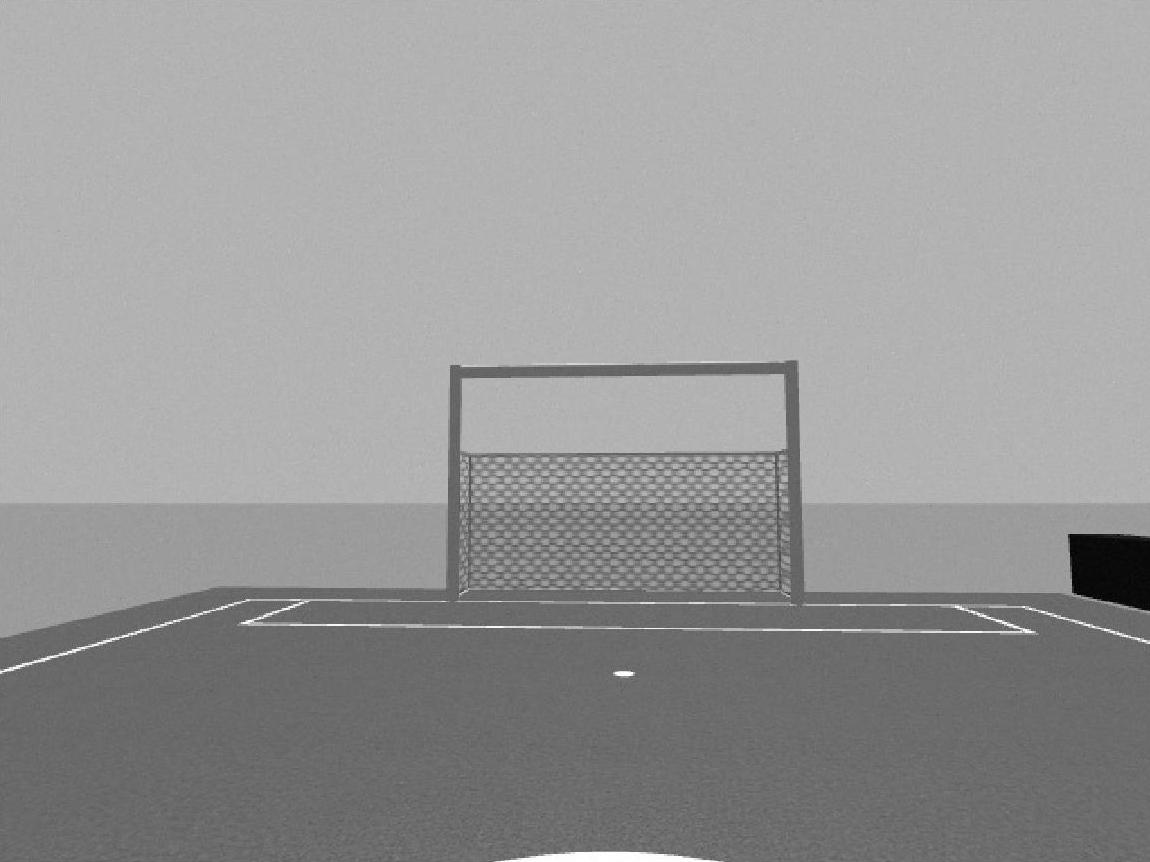
\includegraphics[width=\linewidth]{images/original.jpg}
		\caption{Imagen original}
	\end{subfigure}
	\begin{subfigure}[b]{0.41\linewidth}
		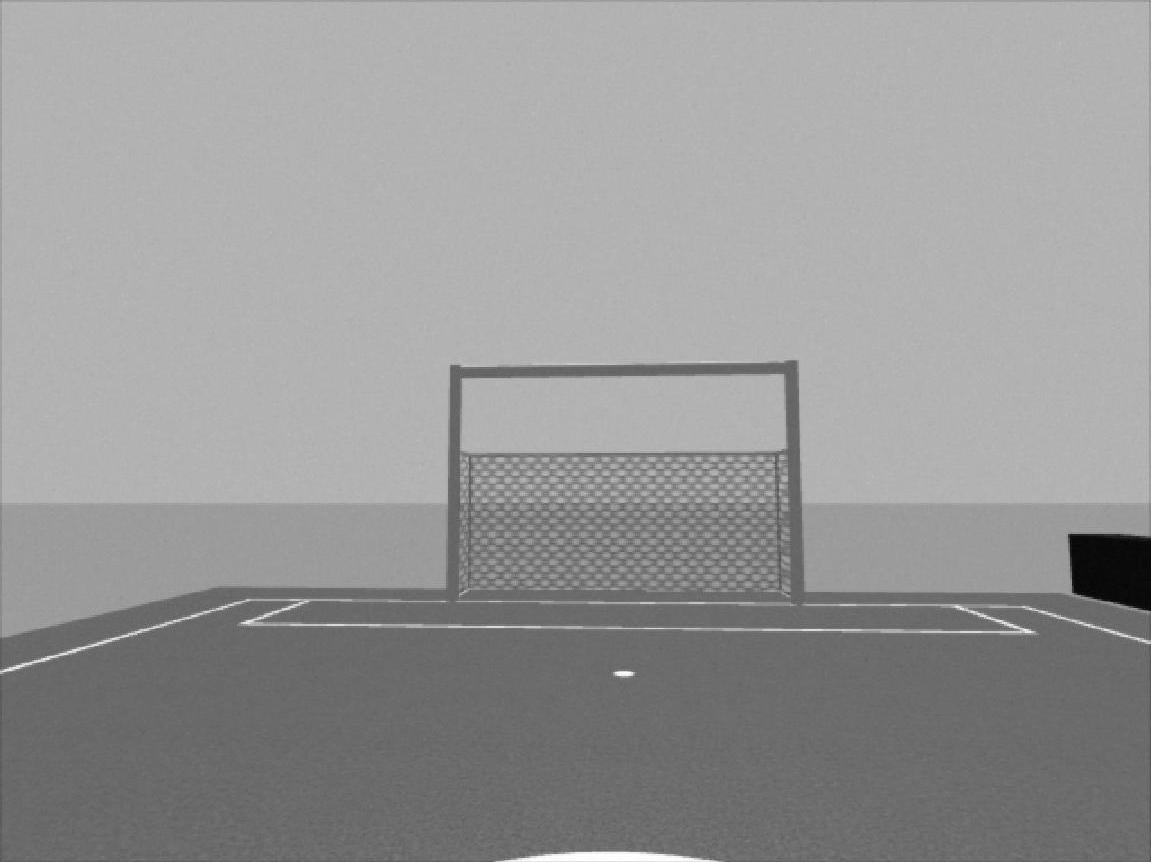
\includegraphics[width=\linewidth]{images/0.5-3.jpg}
		\caption{$\sigma=0.5$}
	\end{subfigure}
	\begin{subfigure}[b]{0.41\linewidth}
		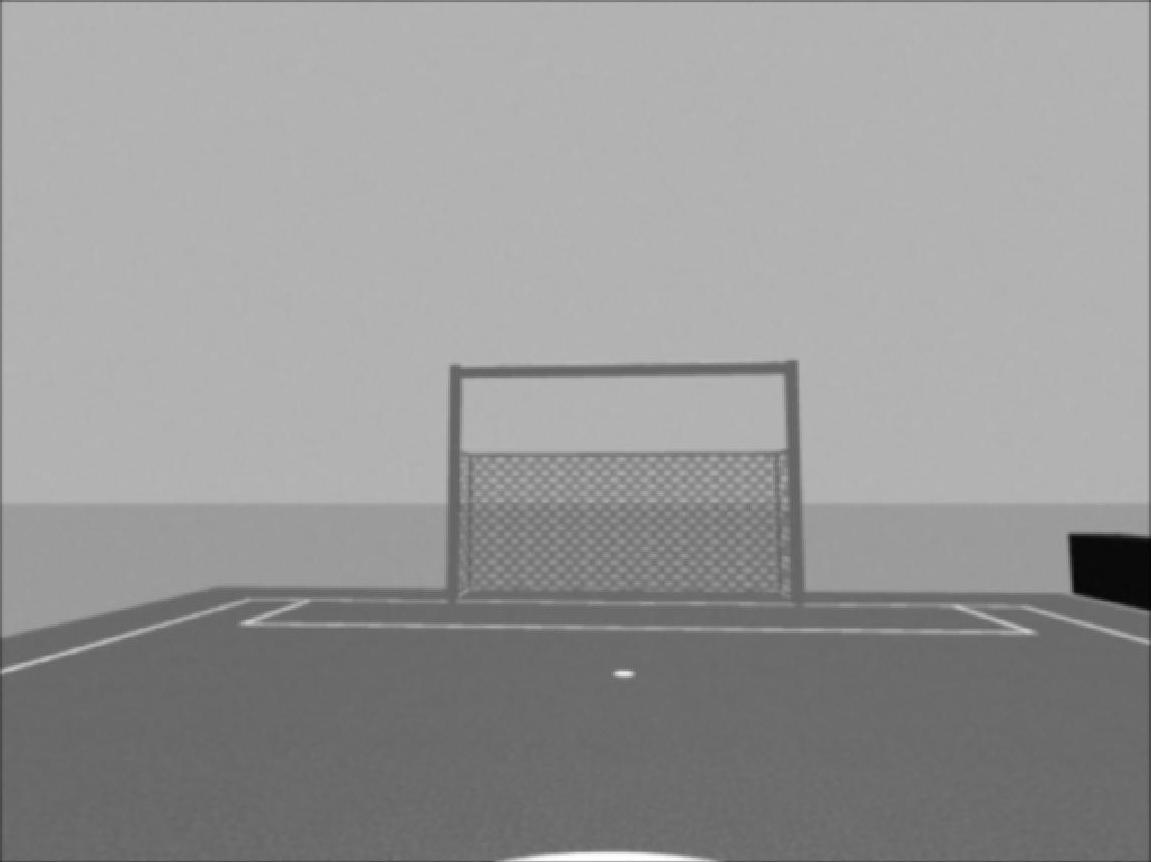
\includegraphics[width=\linewidth]{images/1-5.jpg}
		\caption{$\sigma=1$}
	\end{subfigure}
	\begin{subfigure}[b]{0.41\linewidth}
		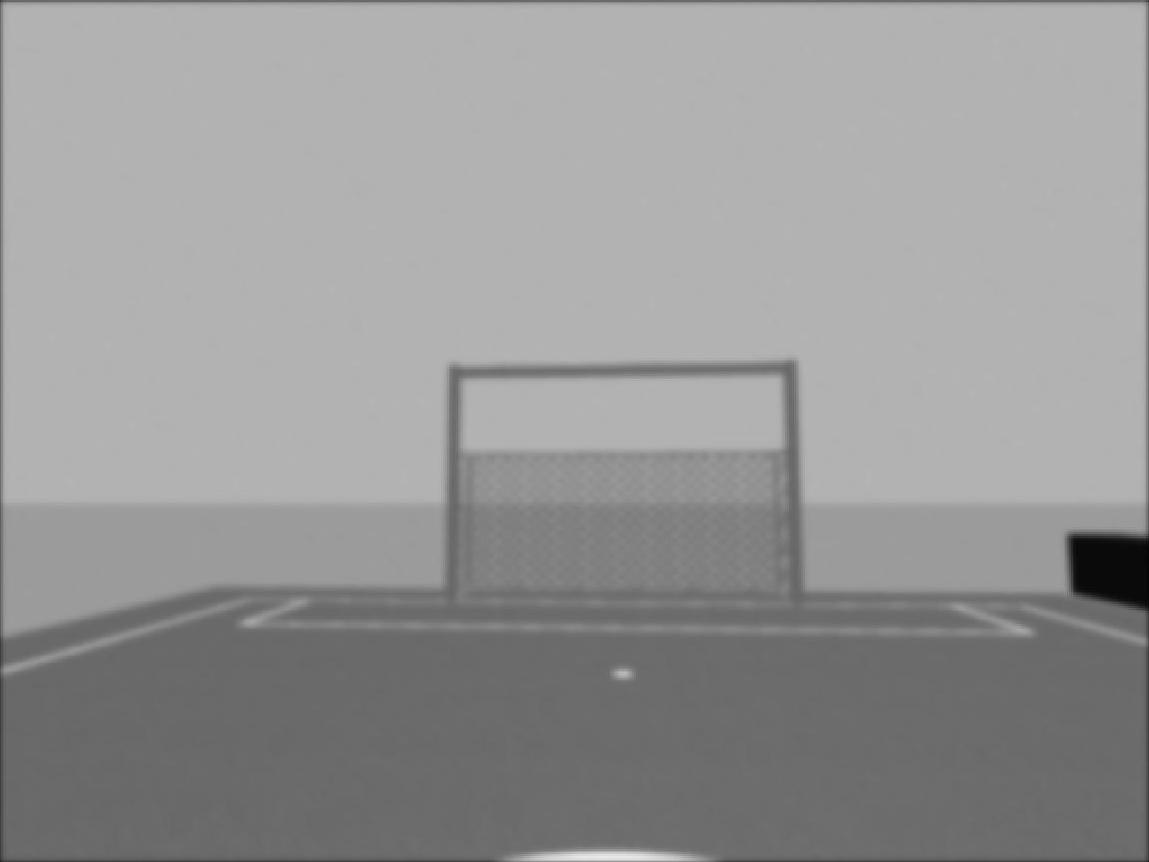
\includegraphics[width=\linewidth]{images/2-13.jpg}
		\caption{ $\sigma=2$}
	\end{subfigure}
	\caption{Filtro gaussiano aplicado en MATLAB variando el valor de sigma.}
	\vspace{1cm}
	\begin{minipage}[b]{0.5\linewidth}
		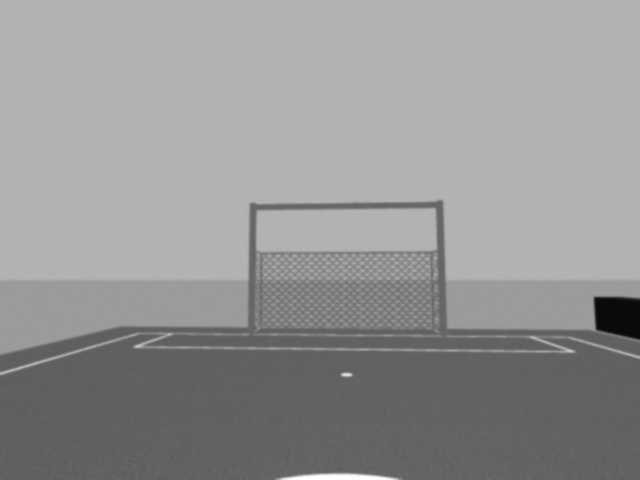
\includegraphics[width=\linewidth]{images/gaussianfilter.jpg}
	\end{minipage}%
	\hspace{1em}
	\begin{minipage}[b]{0.4\linewidth}
		\caption{Al emplear la función \texttt{cv2.GaussianBlur} de OpenCV con un tamaño de 7x7 y un valor de $\sigma=1$, se obtiene como resultado la figura mostrada. Estos parámetros permiten suavizar la imágen de manera efectiva, minimizando el desenfoque y preservando los bordes de la portería.}
	
	\end{minipage}
	\label{fig:sigma}
\end{figure}









\section{Detección de bordes}
%qué es detecc de bord, canny fig y ejemplo con los resultados de ahorita
%A second use for image filtering is to locate places in the image where the intensity
%changes abruptly.
La detección de bordes es importante en el área de procesamiento de imágenes, ya que facilita diversas tareas. Consiste en el análisis de los cambios bruscos en la intensidad de los píxeles para obtener información precisa sobre las regiones de interés.\cite{rebaza2007deteccion} El algoritmo de Canny es usado para detectar todos los bordes que puedan ocurrir en una imagen y es considerado uno de los mejores métodos de detección de contornos \\

\subsection{El Marr-Hildreth Edge Detector\\}
\section{Detección de contornos}

\section{Caracterización de formas}
Los momentos de Hu, 

\section{Estimación de orientación}